% Methodology: Pipeline Architecture
% Author: Adnan Ghribi

\label{sec:methodology}

The proposed pipeline follows a progressive architecture that incrementally increases in complexity and specificity across multiple steps (Fig.~\ref{fig:pipeline_overview}). This design philosophy offers several advantages:

\begin{itemize}
    \item \textbf{Modularity}: Each step is independently optimizable, facilitating debugging, performance tuning, and incremental deployment.
    \item \textbf{Progressive Learning}: Simpler unsupervised methods establish baselines before supervised methods refine predictions.
    \item \textbf{Multi-Objective Optimization}: Different steps target different objectives (early fault-onset detection, fault classification, root cause, subtype clustering), each optimized with appropriate metrics.
    \item \textbf{Interpretability}: Step-wise decomposition enables targeted explainability analysis at each decision point.
\end{itemize}

\begin{figure*}[t]
    \centering
    \includegraphics[width=\textwidth]{example-image}
    \caption{Complete phased pipeline architecture, showing data flow from raw LLRF signals through preprocessing, feature engineering, precursor detection, classification, root cause identification and fault subtype clustering. Each step outputs intermediate results used by subsequent steps.} % MANUAL: placeholder -- author will produce this diagram by hand; the stale pre-V6 figures/pipeline.pdf was removed rather than reused
    \label{fig:pipeline_overview}
\end{figure*}

\subsection{Data Loading and Preprocessing}

Binary LLRF event files are loaded using a dedicated PyPostMortem library (\texttt{programmes/PyPostMortem}). Pre-processing is then applied: completeness/validity checking against the ground-truth classifier's own physics thresholds (Sec.~\ref{sec:system_description}), high-pass filtering, temporal alignment to each event's own true trigger sample index, and Z-score normalization.

\subsubsection{High-Pass Filtering}

In superconducting RF cavities, the measured detuning and microphonics signals contain both fast dynamical components and slow variations originating from mechanical and electromagnetic effects. In particular, DC offsets and low-frequency drifts can arise from Lorentz force detuning, slow mechanical relaxation of the cavity structure, and pressure fluctuations in the cryogenic and vacuum systems. These contributions do not carry information about rapid cavity dynamics but can significantly bias downstream feature extraction.

To suppress these slow components while preserving physically relevant transient phenomena, a 4th-order high-pass Butterworth filter is applied, with a normalized cutoff of 0.01 (relative to each file's own Nyquist frequency -- since the decimation factor, and therefore the effective sampling rate, varies by roughly 250$\times$ across the corpus, Sec.~\ref{sec:system_description}). For numerical implementation, the filter is applied in second-order-sections form via \texttt{scipy.signal.butter(4, 0.01, 'highpass', output='sos')}. % MANUAL: filter order/cutoff/implementation verified directly from prepare_data_cluster_v6.py's scipy.signal.butter() call, a code constant not a manifest metric

\subsubsection{Temporal Alignment}

Each event is aligned to its own true trigger sample index, derived from the acquisition's own time axis rather than a fixed sample offset. An earlier version of this pipeline assumed a fixed offset (sample index 3000) that was wrong for the large majority of files -- the true trigger index varies from roughly 3000 to over 2 million samples depending on the file's own decimation factor and record length. \texttt{Read\_Signals} already returns a correct per-file time axis; the corrected pipeline uses it directly rather than discarding it. % MANUAL: verified against prepare_data_cluster_v6.py module docstring and _v4.py's fix, code facts not manifest metrics

\subsubsection{Per-Event Signal Normalization}

The signals provided by the LLRF instrumentation exhibit heterogeneous physical units and characteristic amplitudes. Direct use of these signals in data-driven models would introduce artificial biases, since variables with larger numerical scales could dominate the learning process independently of their physical relevance. Each signal $s_i(t)$ within a single event is standardized using a Z-score transformation over that event's own full trace,
\begin{equation}
s_i^{\mathrm{norm}}(t) = \frac{s_i(t) - \mu_i}{\sigma_i},
\end{equation}
where $\mu_i$ and $\sigma_i$ denote the mean and standard deviation of signal $i$ within that one event. This is a per-event, per-signal operation with no train/test-fold concept -- it never compares across events and cannot leak information between them. One consequence required a fix: a statistical feature computed from this same normalized trace using the identical whole-signal window -- namely each signal's own mean, standard deviation, RMS, and energy -- would be close to a constant by construction ($\approx 0$, $\approx 1$, $\approx 1$, and a record-length proxy respectively, up to floating-point precision), since that window is exactly the one whose own mean/std defined the normalization. Found during external review, this affected 65 of the previous \MetricZeroSixBinaryClassificationNFeatures{}-feature set (verified directly: near-zero variance across all \MetricZeroZeroDataAttritionChainVSixTotalEvents{} events). \texttt{preprocess\_signals()} now also retains the filtered-but-unnormalized trace, and \texttt{engineer\_features()} computes mean/std/rms/energy from that instead, leaving every scale/shift-invariant statistic (skewness, kurtosis, extrema, quartiles, crest factor, peak count, zero crossings, autocorrelation) on the normalized signal as before; the dataset was re-extracted and every downstream step rerun. This reduced the count of near-constant features in the final set from 65 to 15: two absolute-threshold features (a reflected-signal saturation-fraction check and an RF-drive-on flag) use legacy threshold constants that remain miscalibrated to this signal's real amplitude scale even after the fix -- we corrected the normalization-order bug structurally but had no grounds to invent new threshold values, so these two features are still effectively non-functional and are flagged as an open item (Sec.~\ref{sec:conclusion}); the remaining 13 are metadata-derived state flags (LLRF loop closed, beam present) and precursor-window trend statistics on discrete status channels that are plausibly genuinely constant in this corpus rather than a normalization artifact. None of this changes the classification/SHAP headline findings materially -- tree-based importance already assigns negligible weight to near-constant features -- but the corrected feature count (\MetricZeroSixBinaryClassificationNFeatures{}, up from 770) and the physics-group SHAP breakdown (Sec.~\ref{sec:explainability}) both reflect the fixed pipeline. % MANUAL: 65->15 and the specific still-broken/plausibly-genuine feature breakdown were verified directly against the re-extracted features_engineered.pkl, not yet backed by a results-manifest metric

\subsubsection{Feature-Matrix Normalization for Classifiers}

Separately from the per-event signal normalization above, the tabular feature matrix consumed by the classical classifiers (Sec.~\ref{sec:methodology}) is itself standardized before training. Critically, this scaler's $\mu$ and $\sigma$ are computed \emph{only from the training fold of whichever split is currently in use} (\texttt{StandardScaler.fit} on train, \texttt{.transform} on test, Appendix~\ref{appendix:hyperparameters}) -- never from the combined train+test data. An earlier iteration of this pipeline fit the scaler (and a downstream PCA step) on the full dataset before splitting, which let test-fold information leak into the normalization statistics and inflated several early results; this is one of the two leakage sources documented in Sec.~\ref{sec:discussion}. The fix is enforced at the point of consumption -- every analysis script now derives its own leakage-safe, train-fold-only scaling via a shared utility (\texttt{leakage\_safe\_features.py}) rather than touching the pre-scaled/pre-PCA columns saved directly in the feature-extraction pipeline's own output file, which are themselves still fit on the full dataset and remain leakage-tainted; they are not used by any script producing a number reported in this paper. % MANUAL: leakage-source fact and the still-tainted saved columns, cross-referenced against Sec 7 and leakage_safe_features.py's own docstring rather than a manifest metric

\subsubsection{Temporal Segmentation of Precursor Signals}

To capture the evolution of cavity behavior leading up to fault events, the fixed pre-trigger window used by the early-fault-onset-detection task ($N_{\mathrm{pre}} = 3000$ samples, $\approx$34\,ms at the dominant NDEC=200 decimation setting, Appendix~\ref{appendix:features}) % MANUAL: PRECURSOR_WINDOW_MS / REFERENCE_DT_US code constants, not manifest metrics
is divided into five equal-duration segments. Table~\ref{tab:temporal_segmentation} summarizes the segmentation in terms of sample indices and corresponding time ranges; these segment-level statistics (mean, std, linear trend per segment, Appendix~\ref{appendix:features}) are part of the feature set, allowing the model to distinguish early-window from late-window behavior within the same fixed physical duration.

\begin{table*}[t]
\centering
\caption{Temporal segmentation of the pre-trigger window (NDEC=200, the dominant case, $\Delta t \approx 11.4~\mu$s -- Appendix~\ref{appendix:hyperparameters}).} % MANUAL: REFERENCE_DT_US code constant, not a manifest metric
\label{tab:temporal_segmentation}
\begin{tabular*}{\linewidth}{@{\extracolsep{\fill}}@{}l l@{} l@{}}
\toprule
Segment & Samples & Time Range \\
\midrule
Early      & 0--600       & $T-34$ ms to $T-27$ ms \\ % MANUAL: sample/time boundaries derived from N_pre=3000 split into 5 equal segments at dt=11.36us (REFERENCE_DT_US), not a manifest metric
Mid-Early  & 600--1200    & $T-27$ ms to $T-20$ ms \\ % MANUAL: same derivation as above
Mid        & 1200--1800   & $T-20$ ms to $T-14$ ms \\ % MANUAL: same derivation as above
Mid-Late   & 1800--2400   & $T-14$ ms to $T-7$ ms  \\ % MANUAL: same derivation as above
Late       & 2400--3000   & $T-7$ ms to $T=0$      \\ % MANUAL: same derivation as above
\bottomrule
\end{tabular*}
\end{table*}

\subsubsection{Temporal Derivatives}

To characterize fast transient dynamics, first and second finite-difference derivatives are computed for each signal,
\begin{equation}
\dot{s}_i(t) \approx \frac{s_i(t+1) - s_i(t)}{\Delta t}, \qquad % MANUAL: finite-difference notation, mathematical indices not a result number
\ddot{s}_i(t) \approx \frac{s_i(t+1) - 2s_i(t) + s_i(t-1)}{(\Delta t)^2}, % MANUAL: finite-difference notation, mathematical indices not a result number
\end{equation}
where $\Delta t$ is each file's own sample spacing, measured directly from its time axis (median of consecutive sample differences) rather than assumed constant -- since, as noted above, the effective sampling rate varies substantially across the corpus. For the dominant NDEC=200 case, $\Delta t \approx 11.4~\mu\mathrm{s}$ ($\approx$88\,kHz). % MANUAL: dt_us / REFERENCE_DT_US verified directly from prepare_data_cluster_v6.py, a code constant not a manifest metric

\subsection{Feature Engineering}

Feature engineering aims to encode physically meaningful information from LLRF and auxiliary signals into quantitative descriptors suitable for machine learning, combining accelerator-physics knowledge with statistical and temporal signal analysis. A total of \MetricZeroSixBinaryClassificationNFeatures{} features are extracted per event, after pairwise-correlation filtering (Appendix~\ref{appendix:features} gives the complete breakdown by category); a restricted subset of \MetricZeroFivePhaseZeroPrecursorNFeatures{} features, using only the fixed pre-trigger window, is used specifically for the early-fault-onset-detection task (Sec.~\ref{sec:system_description} explains why this restriction matters).

\subsubsection{Physics-Informed Features}

Physics-informed features are designed to capture the underlying electromechanical and RF dynamics of superconducting cavities, organized into seven families: effective system decay, detuning, microphonics, RF mismatch, modulator command, phase stability, and RF power flow (Appendix~\ref{appendix:features} lists every feature in each family).

\paragraph{Effective System Decay}

In pulsed RF operation, the decay of the cavity field after RF switch-off is commonly described by an exponential law, from which the loaded quality factor $Q_L$ can be inferred. In the SPIRAL2 context, this interpretation is not directly applicable: the cavities operate in continuous-wave (CW) regime, the LLRF feedback loop remains active during the transient, and the observed decay reflects the collective response of the cavity and the RF system rather than the intrinsic electromagnetic dissipation of the cavity alone. We therefore extract \emph{effective system decay} metrics, modeling the post-trigger cavity voltage as
\begin{equation}
V_{\mathrm{cav}}(t) = V_0 e^{-t/\tau_{\mathrm{eff}}}, % MANUAL: mathematical notation (subscript-0 initial value), not a result number
\end{equation}
with $\tau_{\mathrm{eff}}$ estimated by linear regression in logarithmic space over a post-trigger window of 500 samples ($\approx$5.7\,ms). % MANUAL: decay-window length verified directly from calculate_effective_decay()'s decay_window_samples parameter, a code constant not a manifest metric
Deviations from ideal exponential behavior (fit quality, non-exponentiality) are extracted alongside $\tau_{\mathrm{eff}}$ itself, since in CW operation such deviations may reflect feedback-loop dynamics as much as genuine cavity phenomena.

\paragraph{Detuning}

Detuning describes the frequency mismatch between the RF drive and the cavity resonance, arising primarily from Lorentz force detuning (scaling with the square of the accelerating field) and from microphonics. Under small-signal assumptions, detuning is estimated from the temporal evolution of the cavity phase,
\begin{equation}
\Delta f = \frac{1}{2\pi}\frac{d\phi(t)}{dt}. % MANUAL: mathematical notation (2*pi normalization), not a result number
\end{equation}
By unwrapping the phase and performing linear regression over a pre-trigger window, we extract features quantifying average detuning, microphonics-driven variability, drift rate, and the abrupt frequency shift at the trigger.

\paragraph{Microphonics}

Microphonics correspond to mechanical vibrations that modulate the cavity resonance frequency, typically in the 10--100\,Hz range, associated with cryogenic systems, vacuum pumps, and environmental vibrations. % MANUAL: band range matches the "microphonics_band_power" feature's fixed 10-100 Hz band in the feature-engineering code, not a manifest metric
Spectral analysis of the detrended phase signal yields the RMS phase jitter, dominant vibration frequency, band-limited spectral power, and the sharpness (Q-factor) of the dominant spectral peak.

\paragraph{RF Mismatch}

The difference between the reflected-signal amplitude and the amplifier-output amplitude (two distinct measured quantities -- not the modulator command, which is the drive \emph{demand} rather than a measured output, and is modeled separately below) quantifies impedance mismatch and RF-chain transients. Features include pre- and post-trigger RMS of this amplitude difference, the post-trigger maximum excursion, settling time, and the fraction of samples where the reflected signal saturates, alongside the cavity phase's own standard deviation measured over the same pre-/post-trigger windows (a co-located phase-jitter indicator, not a phase of the amplitude-difference signal itself, which has no phase component).

\paragraph{Modulator Command}

Pre-trigger amplitude and phase statistics of the modulator command signal, and the post-trigger change in each, characterize the RF drive itself rather than the cavity response -- useful for distinguishing a drive-side fault from a cavity-side one.

\paragraph{Phase Stability}

Phase fluctuations translate directly into beam energy spread and longitudinal emittance growth. Phase stability features (RMS jitter, peak-to-peak excursion, low-frequency drift slope, integrated pre-trigger power spectral density) are computed from the pre-trigger phase signal and complement the detuning and microphonics indicators by isolating vibration-dominated or reference-noise-limited regimes.

\paragraph{RF Power Flow}

RF power balance provides information on cavity coupling, loading, and impedance matching. The power reflection ratio $R = P_{\mathrm{refl}}/P_{\mathrm{fwd}}$ % MANUAL: renamed from the conventional voltage-reflection-coefficient symbol Gamma to avoid clashing with its standard meaning (R = |Gamma|^2 for a power ratio); a code/notation fact, not a manifest metric
characterizes matching conditions, while transient variations in forward and reflected power reveal fault-induced perturbations. Extracted features describe mean power levels, the power reflection ratio, the power jump at the trigger, and a power-imbalance RMS metric. These are computed as $P_{\mathrm{fwd}} \propto |U_{ci}|^2$ and $P_{\mathrm{refl}} \propto |A_{Ucr}|^2$ (voltage-amplitude-squared proxies from the input-coupler and reflected-signal channels), not from the directly-monitored \texttt{P fwd}/\texttt{P refl} calibrated power-sensor channels listed in Sec.~\ref{sec:system_description}, which are not currently used by this feature family. % MANUAL: signal names (Uci, A Ucr) and the proportionality relation verified directly against the RF Power Flow block of engineer_features() in prepare_data_cluster_v6.py, not a manifest metric

\subsubsection{Statistical Features}

For each of the 27 monitored signals, 17 statistics are computed over the full event window % MANUAL: real signal/statistic counts, verified against engineer_features(), not manifest metrics
(mean, standard deviation, skewness, kurtosis, min/max/range, quartiles/IQR, RMS, crest factor, peak count, energy, zero crossings, lag-1 autocorrelation -- Appendix~\ref{appendix:features}). % MANUAL: "lag-1" is part of a literal feature name, not a result number
This is by far the largest feature group by count, together with the similarly-large Temporal group (Appendix~\ref{appendix:features}) -- a naive SHAP importance comparison that simply sums by group therefore structurally favors these two groups regardless of how informative any single member feature is, since they outnumber the seven named physics-informed families combined by roughly 20:1: % MANUAL: "20:1" is a rounded summary of the exact macro-cited counts on the next line, not a separate manifest metric
\MetricOneZeroPhysicsGroupShapNFeaturesStatistical{} + \MetricOneZeroPhysicsGroupShapNFeaturesTemporal{} vs.\ \MetricOneZeroPhysicsGroupShapNFeaturesEffectiveDecay{}+\MetricOneZeroPhysicsGroupShapNFeaturesDetuning{}+\MetricOneZeroPhysicsGroupShapNFeaturesMicrophonics{}+\MetricOneZeroPhysicsGroupShapNFeaturesRfMismatch{}+\MetricOneZeroPhysicsGroupShapNFeaturesModulatorCommand{}+\MetricOneZeroPhysicsGroupShapNFeaturesPhaseStability{}+\MetricOneZeroPhysicsGroupShapNFeaturesRfPowerFlow{}$={}$\MetricOneZeroPhysicsGroupShapNFeaturesPhysicsInformedTotal{}. We therefore report per-feature-mean SHAP importance, not the group sum, as the primary physics-group metric; the resulting per-category breakdown is presented in Sec.~\ref{sec:explainability}.

\subsubsection{Temporal and Derivative Features}

Temporal features characterize the dynamical evolution of signals through the per-segment slopes (Sec.~\ref{sec:methodology}, Temporal Segmentation above), finite-difference derivatives (above), CUSUM change-point statistics, and early/late-window comparison ratios described in full in Appendix~\ref{appendix:features}.

Overall, the combination of physics-informed, statistical, and temporal features yields a high-dimensional representation of cavity behavior in which physically interpretable descriptors coexist with data-driven signal characterizations.

\subsection{Unsupervised Baselines for Early Fault-Onset Detection}

As part of the early-fault-onset-detection step, several unsupervised anomaly-detection methods are run on the same fixed pre-trigger feature subset as the supervised classifier below, to establish how much of the task's separability is detectable without labels:

\begin{enumerate}
    \item \textbf{Isolation Forest}: scores anomalies by decision-tree isolation path length -- shorter paths indicate anomalies, as outliers are isolated in fewer splits.
    \item \textbf{Local Outlier Factor (LOF)}: compares each point's local density to its k-nearest neighbors' density.
    \item \textbf{Mahalanobis distance}: computed against a Ledoit-Wolf shrinkage covariance estimate on a PCA-reduced representation of the training fold.
    \item \textbf{PCA reconstruction error}: distance between each point and its reconstruction from a training-fold-fit PCA retaining 95\% variance. % MANUAL: hyperparameter constant, verified directly from pipeline/00_scripts/prepare_05_phase0_precursor.py, not a manifest metric
    \item \textbf{DBSCAN}: a transductive density-based outlier flag, fit and scored on the test fold directly (Appendix~\ref{appendix:hyperparameters}).
\end{enumerate}

An ensemble score is formed as the unweighted mean of the min-max-normalized scores from all of the above plus the supervised Random Forest's own probability output. Hyperparameter settings for every method are detailed in Appendix~\ref{appendix:hyperparameters}; score distributions are shown in Fig.~\ref{fig:phase04_scores} and results are reported in Sec.~\ref{sec:results}.

\begin{figure}[t]
    \centering
    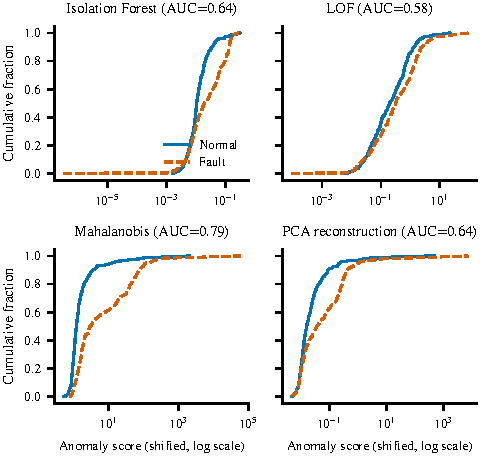
\includegraphics[width=\linewidth]{figures/precursor_unsupervised_scores.pdf}
    \caption{Empirical CDFs of anomaly scores (Isolation Forest, LOF, Mahalanobis, PCA-reconstruction) for the early-fault-onset-detection unsupervised baselines, Normal vs. Fault, on the fixed pre-trigger feature subset. ECDFs rather than histograms: these scores are heavy-tailed, so a linear-axis histogram either hides the bulk of the distribution behind a few extreme outliers or clips them away.} % MANUAL: ECDF/heavy-tail design rationale, not a result number
    \label{fig:phase04_scores}
\end{figure}

\subsection{Early Fault-Onset Detection}

The corrected pipeline trains a Random Forest classifier to identify fault precursors using only the fixed pre-trigger window ($T-34$~ms to $T=0$, % MANUAL: same PRECURSOR_WINDOW_MS code constant as Sec. 3/4 above
restricted to the \MetricZeroFivePhaseZeroPrecursorNFeatures{}-feature true-precursor subset, Sec.~\ref{sec:system_description}), with binary labels indicating post-trigger fault occurrence. Class weights are balanced to handle the imbalanced precursor-vs-normal event distribution (Appendix~\ref{appendix:hyperparameters}). ROC performance and the leading features are shown in Fig.~\ref{fig:phase05_roc} and Fig.~\ref{fig:phase05_importance}; results, including the direct lead-time measurement and its right-censoring, are reported in Sec.~\ref{sec:results}.

\begin{figure}[t]
    \centering
    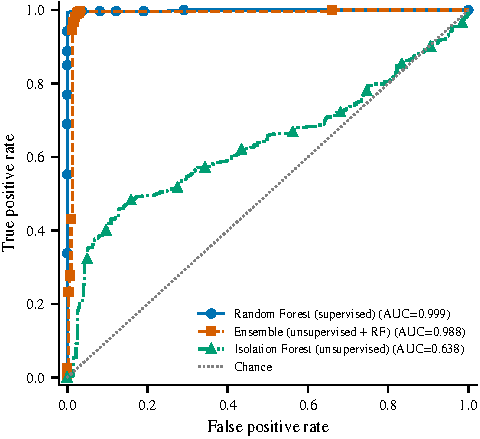
\includegraphics[width=\linewidth]{figures/precursor_roc_curves.pdf}
    \caption{ROC curves for early fault-onset detection: the supervised Random Forest against the unsupervised ensemble and a genuinely unsupervised Isolation Forest baseline, on the same fixed pre-trigger feature subset.}
    \label{fig:phase05_roc}
\end{figure}

\begin{figure}[t]
    \centering
    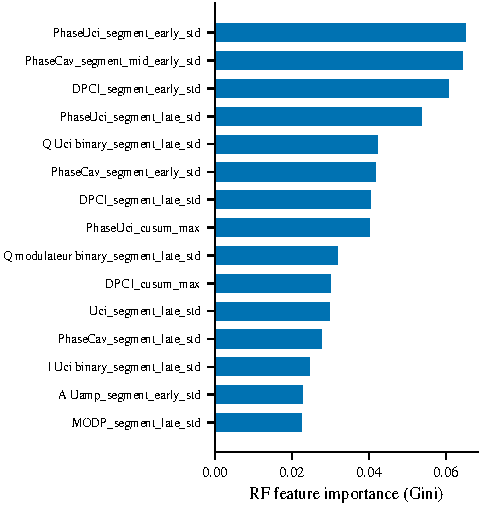
\includegraphics[width=\linewidth]{figures/precursor_feature_importance.pdf}
    \caption{Top 15 Random Forest feature importances (Gini) for early fault-onset detection, restricted to the fixed pre-trigger feature subset (Appendix~\ref{appendix:features}).} % MANUAL: "15" is the figure's own top-N cutoff, a display choice not a manifest metric
    \label{fig:phase05_importance}
\end{figure}

\subsection{Binary Classification}
\label{sec:binary_classification}

Binary classification (fault vs. normal) is performed on the pre-trigger-only \MetricZeroFivePhaseZeroPrecursorNFeatures{}-feature "true precursor" subset (Sec.~\ref{sec:system_description}) -- this, not a full-window version, is the operationally meaningful formulation of the task, since a real-time system only has pre-trigger information available before the interlock trips. Logistic Regression, Random Forest, XGBoost, and SVM (RBF kernel) are compared; this task's classes are close to balanced (Sec.~\ref{sec:introduction}), so no class weighting is applied at this stage (Appendix~\ref{appendix:hyperparameters}). For contrast only, we also report the naive full-window version (post-trigger included, the complete \MetricZeroSixBinaryClassificationNFeatures{}-feature set): its near-ceiling performance is expected and not evidence of a leak, since the full post-trigger window includes the interlock-trip transient by construction, close to trivially separable from normal operation on amplitude alone -- but that formulation was never the operationally meaningful question, and is not the primary result (Sec.~\ref{sec:results}).

\subsubsection{Signal-Ablation Robustness Check}
\label{sec:signal_ablation}

Pre-trigger-only separability alone does not establish a genuinely independent early-warning signal: the model could still be implicitly reading out the same physical quantity that will eventually trip each category's own deterministic threshold, just slightly before it crosses. To test this directly, for each of the seven fault categories we identified the raw signal(s) \texttt{Classify\_PostMortemFile}'s own detection criterion for that category actually reads (verified directly in \texttt{classification.py}, not assumed from the category name -- Sec.~\ref{sec:system_description}), removed every pre-trigger feature derived from that signal, and re-ran the same category-vs-normal classifier comparison restricted to that category's events (Normal as the comparison class, not the other fault categories). Two categories (\textit{Coupure externe rapide}, \textit{Absence autorisation RF}) have no single defining continuous-threshold signal in the classifier code -- their primary label, like all seven categories', comes from a hardware fault-register bit decode, with only four categories additionally refined by a continuous physics threshold; for these two we instead excluded each of the pipeline's monitored raw signal channels one at a time % MANUAL: "27 monitored LLRF signals" already established in Sec. 1/3 as a system constant, not a separate manifest metric here
and report the resulting range. Results are reported in Sec.~\ref{sec:results}.

\subsection{Multi-Label Classification}
\label{sec:multilabel_classification}

Fault events are labeled with one active category out of the seven in Sec.~\ref{sec:system_description} (by construction of the current ground-truth labeling, exactly one label is ever active per event -- Sec.~\ref{sec:system_description}), formulated as a multi-label problem so the pipeline's architecture generalizes to genuinely simultaneous multi-fault events should they occur in future data. A MultiOutput Random Forest baseline (one classifier per label, class-weighted per label) establishes a reference point (Appendix~\ref{appendix:hyperparameters}); three competing approaches to the same task are additionally compared head-to-head -- Binary Relevance, Classifier Chains, and Label Powerset, each with a Random Forest or XGBoost base estimator and a data-driven class-weighting scheme appropriate to that approach (per-label \texttt{class\_weight} for Binary Relevance, an aggregate \texttt{scale\_pos\_weight} for the XGBoost chains, and 'balanced' \texttt{sample\_weight} over powerset classes for Label Powerset -- Appendix~\ref{appendix:hyperparameters}), plus four deep multi-head architectures (CNN, Transformer, CNN-LSTM, MLP) sharing a common per-label \texttt{BCEWithLogitsLoss} with a per-label \texttt{pos\_weight}. Sec.~\ref{sec:results} reports the best-performing approach found (\MetricZeroSevenMultilabelPhaseABCDBestApproach{}), with its headline metric cited as a repeated-split mean $\pm$ std from a live class-weighted rerun (Sec.~\ref{sec:results}); all four deep architectures underperformed the classical baselines on the comparison run of record (Sec.~\ref{sec:discussion}), though that specific deep-architecture comparison has not itself been independently re-verified against a live, class-weighted repeated-split rerun the way Label Powerset has, and should be treated with correspondingly more caution. % MANUAL: cross-references the Table 1 fix (headline Macro-F1 now cites 09_phaseC_lp_stability's live macro instead of a stale pre-class-weighting notebook value) rather than a separate manifest metric

\subsubsection{Pre-Trigger-Only and Unsupervised Evaluation}
\label{sec:multilabel_2x2}

The above comparison uses the full feature set, which includes post-trigger content -- the same question raised for binary classification (Sec.~\ref{sec:binary_classification}) applies here: is any of this separability available before the interlock trip, and is it a genuinely learned decision boundary rather than an artifact only a labeled classifier can reach? We extend the multi-label task along both axes to check. First, the MultiOutput Random Forest baseline and the Binary Relevance/Classifier Chain/Label Powerset comparison are each re-run restricted to the \MetricZeroSixbPhaseOneBinaryPretriggerNFeatures{}-feature pre-trigger-only "true precursor" subset (the same restriction as Sec.~\ref{sec:binary_classification}), completing a supervised comparison across both window conditions.

Second, we built a genuinely unsupervised counterpart to the multi-label task, previously absent from the pipeline, in both window conditions: (1) the four continuous-score anomaly-detection methods from the early fault-onset detection task (Isolation Forest, LOF, Mahalanobis distance, PCA reconstruction error -- Sec.~\ref{sec:methodology}), fit on the training fold and scored on the held-out test fold exactly as in that task, evaluated per fault category as a one-vs-rest ROC AUC against each of the seven \texttt{y\_multilabel} columns independently -- DBSCAN, transductive by construction, contributes a binary outlier flag rather than a continuous score, so it is reported as a per-category outlier-recall diagnostic instead of an AUC, the same exclusion already applied to that task's ensemble score; and (2) K-Means, Agglomerative clustering, and a Gaussian Mixture Model, each fit directly on the full, unsplit dataset -- an internal-structure comparison, not a generalization claim, matching the fault subtype clustering task's own no-train/test-split precedent (Sec.~\ref{sec:methodology}) -- at $k=\MetricZeroSevenbPhaseTwoMultilabelUnsupervisedClusteringK{}$ clusters (the number of distinct categories present: "Normal" plus the seven fault types), then compared against ground truth via Adjusted Rand Index, Normalized Mutual Information, and cluster purity. That ground truth reuses \texttt{prepare\_08\_phase3a\_rootcause.py}'s own \texttt{argmax(y\_multilabel, axis=1)} convention verbatim (Sec.~\ref{sec:rootcause}) rather than defining a separate one; since the current dataset's ground-truth labeling never activates more than one category per event (above), this is an exact category assignment here, not the lossy simplification it would be for genuinely simultaneous multi-fault events. DBSCAN's neighborhood radius (\texttt{eps}) is auto-tuned per run from a 75th-percentile-of-5-nearest-neighbor-distance heuristic -- the same one the fault subtype clustering task already uses (Sec.~\ref{sec:methodology}) -- rather than a fixed value carried over from a different feature space, after an initial run with a fixed \texttt{eps} (copied from the early fault-onset detection task) proved uninformative: it flagged every single test event as an outlier in both window conditions, a degenerate result from a hyperparameter that did not transfer, not a finding. Results for both extensions are reported in Sec.~\ref{sec:results}. % MANUAL: "(1)"/"(2)" are a two-item enumeration, not results; "08" is a literal script-filename fragment (prepare_08_phase3a_rootcause.py); "75th-percentile-of-5-nearest-neighbor" is a literal, fixed hyperparameter-heuristic description (matching prepare_09_phase3b_clustering.py's own NearestNeighbors(n_neighbors=5)/np.percentile(..., 75) code), not a manifest metric

\subsection{Root Cause Identification}
\label{sec:rootcause}

For events where multiple fault labels might be simultaneously active, root cause identification asks which is the primary one. We state its ground-truth construction explicitly, since it is a real limitation of the current task formulation rather than a solved comparison (Sec.~\ref{sec:discussion}): the training target is \texttt{np.argmax(y\_multilabel, axis=1)} -- a deterministic rule selecting the first flagged category in bit order, not an independently-labeled physical root cause. % MANUAL: "axis=1" is a literal code argument (prepare_08_phase3a_rootcause.py), not a result number
Because the current dataset contains zero genuinely multi-fault events (Sec.~\ref{sec:system_description}), this target currently has an unambiguous single answer for every event by construction, rather than exercising a tie-breaking rule among multiple active labels.

A class-weighted Random Forest classifier (unlimited depth, Appendix~\ref{appendix:hyperparameters}) is trained on the \MetricZeroSixBinaryClassificationNFeatures{}-feature set to predict the primary fault category among the seven in Sec.~\ref{sec:system_description}, among the \MetricZeroEightPhaseThreeaRootcauseNFaultEvents{} fault events. Headline accuracy and per-category performance (repeated-split mean $\pm$ std, and the resulting severe spread on the rarest categories) are reported and analyzed in Sec.~\ref{sec:results}.

\subsection{Fault Subtype Clustering}

Within each fault category, unsupervised clustering (K-Means, Agglomerative, and Gaussian Mixture, best method selected by silhouette score, Appendix~\ref{appendix:hyperparameters}) is applied independently to discover subtypes potentially corresponding to distinct physical mechanisms or operational conditions. Candidate cluster counts $k \in [2, 6]$ % MANUAL: n_clusters_range=(2,6) default in cluster_within_fault_type(), a code constant
are evaluated, further capped at $\min(k_{\max}, \lfloor n_{\mathrm{category}}/5 \rfloor)$ for small categories (the full $k\in[2,6]$ range is reachable for every one of the six categories with enough events on the current dataset, since the smallest, $n=31$, still permits $k$ up to 6); categories with too few events (below a minimum-event guard in \texttt{cluster\_within\_fault\_type()}) are skipped rather than forced into a fixed cluster count. % MANUAL: the /5 cap divisor is a code constant in cluster_within_fault_type(); n=31 is cavity quench/breakdown's real category size, cross-referenced against Sec. 3's attrition-chain macro elsewhere

Two corrections were required before this result could be trusted, both found while building the feature-profile figure below (Fig.~\ref{fig:phase09_profiles}). First, an unguarded near-zero-denominator division in \texttt{engineer\_features()}'s \texttt{early\_late\_ratio} computation let a handful of events take on extreme values (up to 24 standard deviations from their category mean); we added a proper relative-scale guard and re-extracted the full V6 dataset (Sec.~\ref{sec:system_description}). Second, and more consequentially, even after that fix, selecting the "best silhouette across every candidate (algorithm, $k$) combination" reliably chose whichever candidate isolated the single tightest, most extreme minority subgroup -- as small as one event out of 591 -- rather than a genuine population split: a tight, well-isolated singleton or pair routinely scores higher on silhouette than a fair partition of a more continuous distribution, so unconstrained silhouette maximization is structurally biased toward outlier isolation over real bimodal structure. We therefore winsorize each feature at the 5th/95th percentile within each category before clustering, and only accept a candidate labeling if every resulting cluster holds at least 15\% of that category's events; a category with no candidate meeting this bar is reported as having no established balanced subtype structure rather than falling back to an outlier-driven pick. In practice, five of the \MetricZeroNinecEnhancedSubclassDiscoveryNCategoriesAnalyzed{} analyzable categories (\texttt{prepare\_09c\_enhanced\_subclass\_discovery.py}) produce a balanced $k=2$ split under this constraint; the sixth, \textit{Rég signal RF hors tolérance} -- by far the largest -- does not, discussed below and further in Sec.~\ref{sec:weakness_diagnosis}. % MANUAL: the 15% balance threshold and 5th/95th winsorization percentiles are script constants (cluster_within_fault_type()), not manifest metrics

Table~\ref{tab:subtype_clustering_methodology} shows the corrected result for every category with enough events to analyze. Five converge to the same $k=\MetricZeroNinecEnhancedSubclassDiscoveryRfAuthorizationAbsentBestK$, with the minority cluster holding between 15\% and 42\% of each category's events (real population sizes, not a residual outlier) and a weak-to-moderate silhouette range reflecting a real but not sharply-separated structure -- lower than the pre-correction range, since that range was inflated by the outlier-isolation artifact above rather than genuine separation. % MANUAL: 15%/42% minority-share range computed directly from the corrected best_labels cluster_sizes in the 09c manifest/pickle, not itself an exposed manifest metric
We flag one limitation of the balance constraint itself: requiring every cluster to hold $\geq$15\% of a category's events is arithmetically infeasible for $k\geq7$ and increasingly restrictive as $k$ grows, so it structurally favors small $k$ regardless of the data -- "consistent $k=2$" should be read as "the only balance-feasible outcome across most of the search space" for the categories where a balanced split exists at all, not as an unconstrained data-driven convergence. It is also strict enough to reject real structure outright: a follow-up, unconstrained investigation of the sixth category (Sec.~\ref{sec:weakness_diagnosis}) finds three independent clustering methods agreeing on a genuine $\sim$13\% minority subgroup that simply falls a few points under this floor. % MANUAL: 15% balance threshold and the k>=7 infeasibility point are arithmetic consequences of that same script constant, not separate manifest metrics
We do not yet pair this with a systematic per-subtype physical characterization (Sec.~\ref{sec:conclusion}); Fig.~\ref{fig:phase09_profiles} shows the top differentiating features per category as a first step in that direction.

\begin{table}[t]
\centering
\caption{Fault subtype clustering: best $k$ and silhouette score per category with enough events to analyze (\MetricZeroNinecEnhancedSubclassDiscoveryNCategoriesAnalyzed{} of \MetricZeroNinecEnhancedSubclassDiscoveryNCategoriesTotal{} categories)}
\label{tab:subtype_clustering_methodology}
\begin{tabular*}{\linewidth}{@{\extracolsep{\fill}}@{}lcc@{}}
\toprule
\textbf{Fault category} & \textbf{Best $k$} & \textbf{Silhouette} \\
\midrule
Seuil pick-up & \MetricZeroNinecEnhancedSubclassDiscoveryPickupThresholdBestK & \MetricZeroNinecEnhancedSubclassDiscoveryPickupThresholdSilhouette \\
RF authorization absent & \MetricZeroNinecEnhancedSubclassDiscoveryRfAuthorizationAbsentBestK & \MetricZeroNinecEnhancedSubclassDiscoveryRfAuthorizationAbsentSilhouette \\
Vacuum threshold & \MetricZeroNinecEnhancedSubclassDiscoveryVacuumThresholdBestK & \MetricZeroNinecEnhancedSubclassDiscoveryVacuumThresholdSilhouette \\
Cavity quench/breakdown & \MetricZeroNinecEnhancedSubclassDiscoveryCavityQuenchBreakdownBestK & \MetricZeroNinecEnhancedSubclassDiscoveryCavityQuenchBreakdownSilhouette \\
RF safety threshold exceeded & \MetricZeroNinecEnhancedSubclassDiscoveryRfSafetyThresholdExceededBestK & \MetricZeroNinecEnhancedSubclassDiscoveryRfSafetyThresholdExceededSilhouette \\
RF regulation out of tolerance & no valid split & no valid split \\ % MANUAL: this category's best_k/silhouette are null in the manifest (no candidate satisfied the balance constraint), so no macro exists for them -- see Sec.~\ref{sec:weakness_diagnosis} for the follow-up investigation's real (unconstrained) numbers
\bottomrule
\end{tabular*}
\end{table}

\begin{figure*}[t]
    \centering
    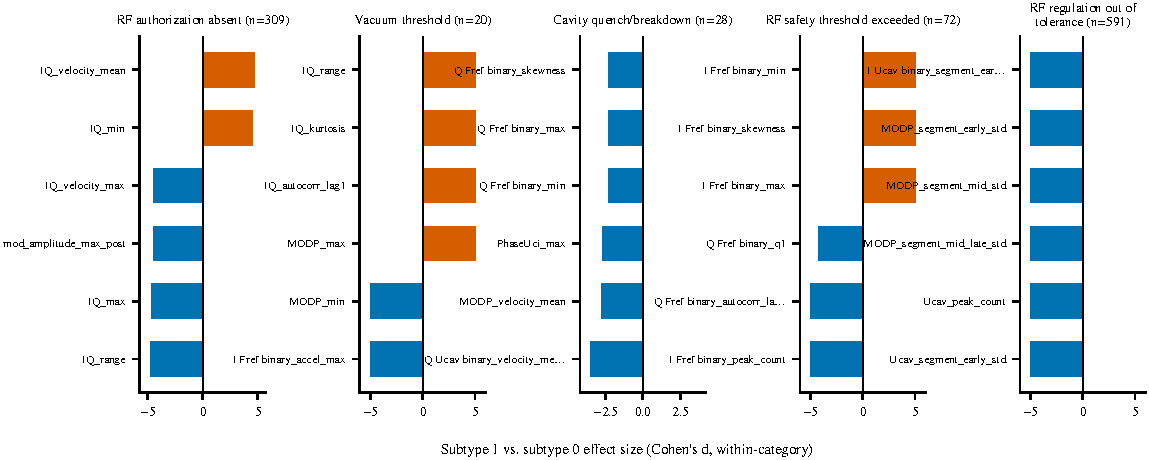
\includegraphics[width=\textwidth]{figures/subtype_feature_profiles.pdf}
    \caption{Top 6 differentiating features per category between the two corrected, balanced subtype clusters (subtype 1 minus subtype 0, Cohen's $d$ within category, computed on the same winsorized representation used for clustering; clipped to $\pm5$ -- beyond that magnitude a handful of near-constant-within-subgroup features would otherwise dominate the scale without being more informative). A first step toward the systematic per-subtype physical characterization noted above (Sec.~\ref{sec:conclusion}), not yet a complete one.} % MANUAL: Cohen's d clip bound and top-N cutoff are figure display choices (report/code/fig_subtype_profiles.py), not manifest metrics
    \label{fig:phase09_profiles}
\end{figure*}

\subsection{Explainability and Reporting}

Every quantitative claim in this report, including every table and macro cited above, is generated from a versioned, git-tracked results manifest (\texttt{analysis/results\_manifest/*.yaml}) rather than hand-typed: each pipeline script writes its own manifest at the end of its run, \texttt{report/code/generate\_macros.py} converts every manifest into a \texttt{\textbackslash Metric...} LaTeX macro, and \texttt{report/code/check\_no\_hand\_typed\_numbers.py} flags any bare numeric literal in the report text that is not backed by such a macro or an explicit \texttt{\% MANUAL:} justification. Re-running an affected pipeline script and then \texttt{make sync} in \texttt{report/} regenerates the macros and re-runs the check, so a future pipeline change is reflected in every citing section automatically rather than requiring a manual re-derivation of every number by hand.
